\documentclass[12pt]{article}

\usepackage{amsmath}
\usepackage{amssymb}
\usepackage{graphicx}
\usepackage[outdir=./]{epstopdf}
\usepackage{setspace}
\usepackage{geometry}
\usepackage{booktabs}
\usepackage{hyperref}
\usepackage{xurl}
\usepackage{float}
\usepackage[expansion=false]{microtype}
\geometry{margin=1in}
\setstretch{1.2}

\title{The Nonlinear Geometry of State-Building: \\Mapping Global Governance Trajectories via Manifold Learning}

\author{
Adriel I. Santoso \\
Department of Mechanical and Aerospace Engineering \\
Tohoku University
}

\date{\today}

\begin{document}

\maketitle

\begin{abstract}
    While comparative political science frequently relies on discrete regime typologies, assuming linear pathways of state development, this paper re-conceptualizes global governance as a continuous dynamical system. Using longitudinal Quality of Government (QoG) data (1990--2026), we construct a global governance phase-space via non-linear Diffusion Maps and Topological Data Analysis (TDA). By projecting decades of historical data onto a 2026 reference manifold using Nyström approximation, we mathematically map the structural constraints of state-building. We introduce two novel macro-political metrics---\textit{Trajectory Tortuosity} and \textit{Geodesic Inefficiency}---to quantify the systemic friction of institutional reform. Unsupervised clustering of these historical trajectories identifies three distinct developmental paradigms: Direct, Meandering, and Erratic. Furthermore, persistent homology identifies severe \textit{Topological Voids}, mathematically proving the existence of structurally ``forbidden zones'' where mismatched economic and institutional configurations invariably collapse. Ultimately, we demonstrate that a state's trajectory through the governance manifold is more analytically significant than its current static classification, directly challenging the viability of static reform conditionality in international development policy.
\end{abstract}

\section{Introduction}

Comparative political science has long debated how states transition between autocracy, democracy, and economic prosperity. However, these debates frequently rely on discrete categorical models---classifying a state as an ``electoral autocracy'' or a ``consolidated democracy.'' While heuristically useful, these static categories fail to capture the fluid, dynamic trajectories states take over time.

If global governance is a complex adaptive system \cite{miller2007complex, simon1962architecture}, countries behave less like specimens pinned to a board and more like an ensemble of particles moving through a continuous mathematical space. This paper bridges formal dynamical systems theory and empirical political science by proposing a geometric framework for state trajectories. We ask: What is the underlying shape of global governance? Do states take efficient, direct paths toward development, or do they wander erratically? And finally, is the global ensemble of states converging toward a single model, or fracturing into distinct topological basins?

\section{Theoretical Context and Literature Review}

\subsection{The Limits of Discrete Typologies}
For decades, comparative political science has heavily relied on discrete categorizations to measure state development. Indices such as Polity IV, Freedom House, and the foundational elements of the Varieties of Democracy (V-Dem) project \cite{coppedge2025vdem} are frequently deployed to sort nations into taxonomic bins: ``closed autocracies,'' ``electoral autocracies,'' or ``consolidated democracies.'' While these discrete typologies are heuristically useful for descriptive statistics and panel regressions, they inherently freeze a dynamic system in time.

The assumption underlying much of the classical ``transition paradigm'' was that states moved along a relatively linear continuum toward democratic consolidation and economic modernization. However, as scholars have increasingly noted, democratic backsliding, stalled transitions, and resilient authoritarianism have disrupted this linear expectation. When a state is classified merely by its current static attributes, the vector and momentum of its institutional development are lost. Two states may temporarily occupy the same ``electoral autocracy'' categorization, yet one might be rapidly collapsing from a prior democratic peak while the other is slowly consolidating bureaucratic capacity. Standard econometric models struggle to differentiate these radically different trajectories because they fail to account for the spatial and temporal continuity of state-building.

\subsection{State-Building as a Complex Adaptive System}
To move beyond static categories, this paper conceptualizes global governance as a complex adaptive system operating within a continuous mathematical space. In this framework, countries are not isolated data points to be categorized, but dynamic entities traversing a multi-dimensional phase-space defined by their institutional, social, and economic parameters.

This approach aligns with recent advances in political economy that view institutional development as highly non-linear. Most notably, Acemoglu and Robinson's concept of the ``Narrow Corridor'' \cite{acemoglu2019narrow} posits that the dual emergence of state capacity (the ``Leviathan'') and societal liberty must co-evolve in a delicate, precarious balance. If state capacity outpaces societal control, the system is pulled toward despotic attractors; if societal fragmentation outpaces state capacity, it collapses into anarchic or deeply inefficient voids.

\subsection{The Geometry of Governance}
Translating the ``Narrow Corridor'' into the language of differential geometry provides a powerful new analytical lens. The viable pathways for state development do not fill the entirety of the theoretical parameter space; rather, they are restricted to a lower-dimensional manifold—a specific geometric surface embedded within the higher-dimensional data. Areas outside this manifold represent structurally unstable or impossible configurations of governance.

By applying manifold learning to longitudinal cross-national data, we can empirically map this corridor. Instead of assuming linear transition paths, we can mathematically calculate the actual "terrain" of global governance. In this topological space, stable institutional arrangements act as gravity wells or ``attractors,'' while highly unstable configurations act as ``repulsors'' or ``topological voids.'' Evaluating a state's trajectory through this geometric landscape allows us to measure not just where a state is, but how efficiently it is moving through the permissible pathways of institutional development.

\section{Methodology}

To map the dynamical system of global governance, we establish a continuous, low-dimensional reference geometry that represents the ``permissible'' configurations of state development. We then project longitudinal time-series data onto this geometry to track national trajectories.

\subsection{Data Acquisition and Preprocessing}
We utilize the Quality of Government (QoG) Standard Dataset \cite{teorell2026qog}, combining cross-sectional data (for manifold construction) and time-series data from 1990 to 2026 (for trajectory projection). The post-1990 timeframe is specifically chosen to capture the institutional dynamics following the end of the Cold War and the ``Third Wave'' of democratization.

We analyze state configurations across six dimensions. To capture core institutional frameworks, we rely on the Varieties of Democracy (V-Dem) project: Electoral Democracy (\textit{vdem\_polyarchy}), Egalitarian Component Index (\textit{vdem\_egal}), and Political Corruption (\textit{vdem\_corr}). To capture structural modernization, we utilize World Development Indicators (WDI): Urbanization (\textit{wdi\_popurb}), Life Expectancy (\textit{wdi\_lifexp}), and Logged GDP per Capita.

Missing values were imputed using a $K$-Nearest Neighbors ($K=5$) approach. In global governance datasets, missingness is structurally non-random; highly authoritarian or collapsing regimes systematically suppress data. Utilizing listwise deletion would artificially truncate the autocracy end of the parameter space, introducing severe selection bias into the underlying geometry.

\subsection{Variable Selection and Manifold Stability}
Feature selection in high-dimensional political datasets often suffers from severe collinearity, where including redundant variables artificially inflates the topological weight of specific concepts. To avoid this, we utilized a theoretically constrained 6-variable feature space: three core institutional metrics and three structural modernization proxies.

To rigorously validate that this selection does not introduce arbitrary geometric distortion, we performed a Procrustes sensitivity analysis. We constructed a purely institutional ``baseline'' manifold using only the V-Dem variables, and calculated its geometric alignment against our expanded 6-variable model using orthogonal Procrustes rotation. The coordinate alignment was exceptionally strong ($r = 0.9020$), demonstrating that the primary political topology remains highly stable. Conversely, introducing redundant developmental indices (such as the UNDP Human Development Index \cite{undp2024hdi}) immediately degraded manifold stability ($r = 0.8528$) due to collinearity with existing wealth and health metrics. Thus, our 6-variable model optimizes the balance between theoretical institutional mapping and structural economic realities.

\subsection{The Reference Manifold: Why Diffusion Maps?}
Standard dimensionality reduction techniques are ill-suited for analyzing state trajectories. Principal Component Analysis (PCA) assumes linear relationships, which fails to capture the curving ``corridors'' of state-building. Modern manifold learning tools like t-SNE or UMAP are optimized for visual clustering, but they frequently distort global distances and density, making them mathematically invalid for measuring travel distance over time.

Instead, we utilize Diffusion Maps, a non-linear spectral technique that preserves local transition probabilities \cite{coifman2006diffusion}. Diffusion Maps conceptualize the data space as a physical system where a random walk (or diffusion process) occurs. Given our dataset $X = \{x_1, ..., x_n\}$, we construct a weighted adjacency matrix using a Gaussian kernel:
$$W_{ij} = \exp\left(-\frac{\lVert x_i - x_j \rVert^2}{2\epsilon^2}\right)$$

where $\epsilon$ is the kernel bandwidth, empirically set to the median pairwise distance ($\epsilon = 2.8754$). We define a diagonal normalization matrix $D$ where $D_{ii} = \sum_j W_{ij}$, and compute the symmetric Markov transition matrix:
$$A = D^{-1/2} W D^{-1/2}$$

The eigenvectors of $A$ provide a stable coordinate system. Because Diffusion Maps are built on Markov chains, distance in this space directly correlates to the probability of transitioning from one state of governance to another.

\subsection{Topological Data Analysis and Persistent Homology}
While Diffusion Maps reveal the shape of the data, Topological Data Analysis (TDA) allows us to study the ``holes'' in that shape \cite{carlsson2009topology}. Standard statistics focus on where data \textit{is}; TDA allows us to mathematically prove where data \textit{cannot be}.

Using persistent homology, we construct a Vietoris-Rips complex across our high-\hspace{0pt}dimensional space. We measure Betti numbers, specifically the zeroth Betti number ($H_0$), which counts connected components, and the first Betti number ($H_1$), which counts structural loops or voids. In the context of political economy, an $H_1$ void represents a ``forbidden zone'' or an inherently unstable regime configuration. If a topological hole exists, it implies that a state attempting to adopt the institutional attributes of that region will face overwhelming systemic pressure to collapse toward the edges of the void.

\subsection{Historical Projection and Trajectory Metrics}
To analyze how states navigate this geometry, historical time-series data (1990--2026) is projected onto the static reference manifold using a Nyström extension. This prevents historical volatility from warping the underlying geometric terrain. We introduce two macro-po\-lit\-i\-cal metrics to quantify the institutional ``friction'' or ``wasted effort'' of a state's development over $N$ time steps.

The first metric, \textbf{Trajectory Tortuosity ($T$)}, represents the ratio of the total Euclidean path length traversed over the net displacement \cite{benhamou2004reliably}. This measures how directly a state achieved its current governance configuration and is formally defined as:
$$T = \frac{\sum_{t=1}^{N-1} \lVert x_{t+1} - x_t \rVert}{\lVert x_N - x_1 \rVert}$$

The second metric, \textbf{Geodesic Inefficiency ($I$)}, accounts for the fact that pure Euclidean space ignores the manifold's actual shape. While Euclidean distance measures a straight line, geodesic distance respects the ``terrain'' of allowable governance. We compute the shortest path $G$ through a $k$-NN graph of the manifold and define inefficiency as $I = \frac{G}{L}$, where $L$ is the Euclidean length. This metric isolates the specific cost of instituting reforms that move \textit{against} the natural grain of the systemic landscape.

To account for the extreme right-skew inherent to ratio bounds, both $T$ and $I$ undergo a logarithmic transformation before being subjected to unsupervised $K$-Means clustering to organically identify macroscopic trajectory paradigms.

\section{Empirical Results}

\subsection{The Shape of Governance and Topological Voids}
Spearman correlation diagnostics reveal the empirical nature of the diffusion manifold. The primary gradient (Axis 1) strongly correlates with egalitarianism (+0.877) and control of corruption (-0.890), representing a continuum of \textbf{Socio-Institutional Capacity}. Axis 2 correlates positively with urbanization (+0.645) and wealth (+0.442) but negatively with democracy (-0.349), capturing an axis of \textbf{Autocratic Modernization}.

\begin{figure}[htbp]
    \centering
    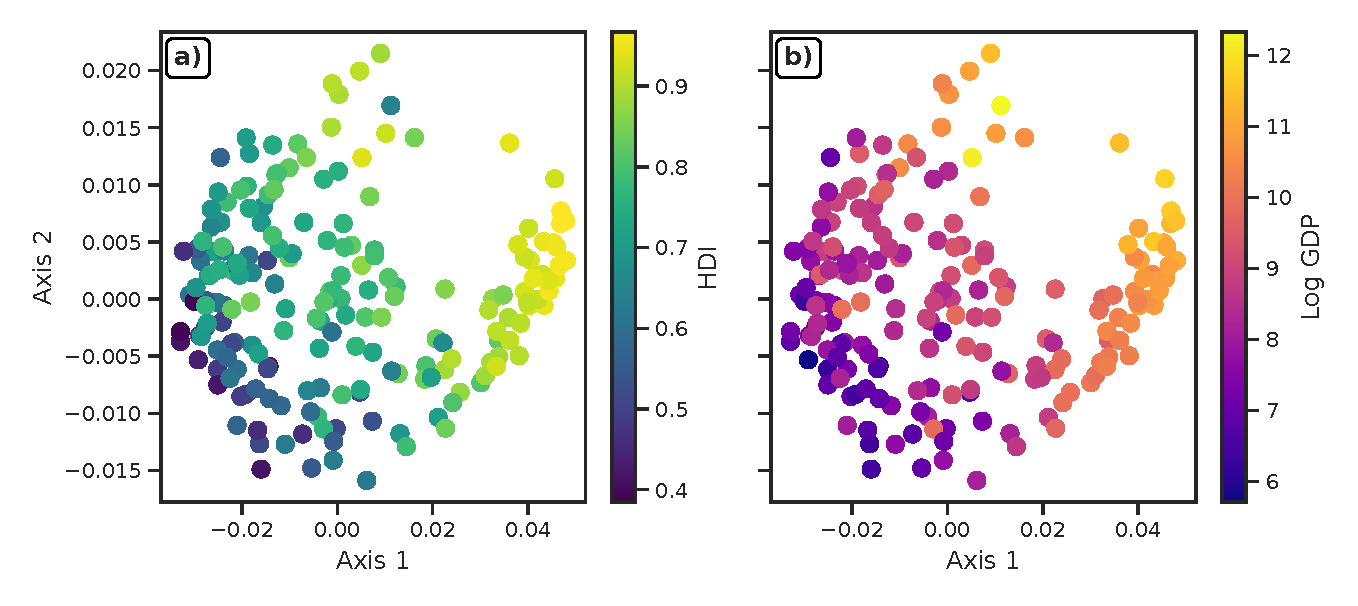
\includegraphics[width=0.95\textwidth]{../figures/fig1_reference_manifold.eps}
    \caption{\textbf{The Reference Manifold.} A side-by-side comparison of the 2026 governance manifold. \textbf{a)} Colored by HDI, the manifold reveals a smooth developmental gradient across Socio-Institutional Capacity (Axis 1). \textbf{b)} Colored by Log GDP, it illustrates the ``rentier state anomaly,'' where natural resource wealth pulls states upward along the Autocratic Modernization gradient (Axis 2) without corresponding institutional progress.}
    \label{fig:manifold}
\end{figure}

To prove the existence of structural boundaries within this space, we apply persistent homology (TDA) to the high-dimensional feature set. The persistence barcode (Figure 2) reveals 40 distinct $H_1$ loops. These topological voids mathematically prove the existence of ``forbidden zones'' in state development, indicating macro-level combinations of governance variables that are geometrically impossible to sustain.

By calculating the multidimensional density gradient and isolating the bounds of the primary persistent void, we identify a distinct structural hole. This void is bounded by states with moderately high wealth (mean GDP per capita of \$34,648) and urbanization (61.6\%), but critically low democratic freedoms (polyarchy index 0.33) and high corruption levels (0.49). The topology mathematically demonstrates that a state cannot persist in this specific high-wealth/high-corruption configuration indefinitely; the system forces a systemic collapse either toward institutional reform or economic degradation.

\begin{figure}[htbp]
    \centering
    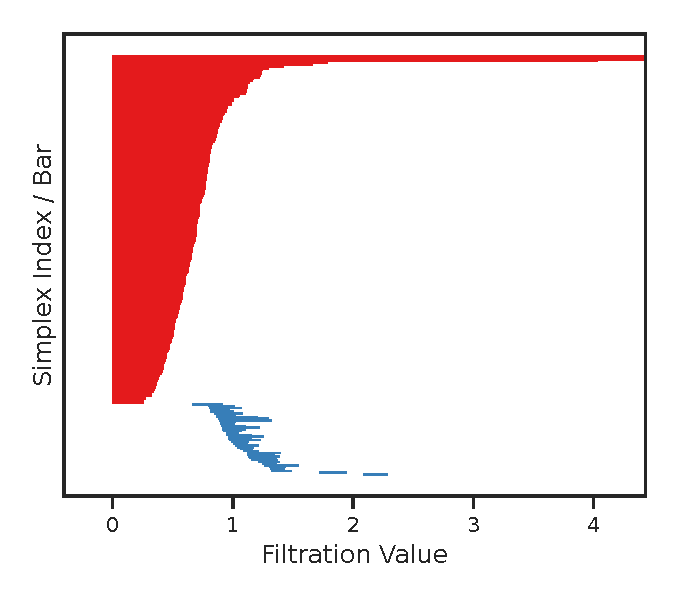
\includegraphics[width=0.5\textwidth]{../figures/fig2_persistence_barcode.eps}
    \caption{\textbf{Persistence Barcode.} TDA of the high-dimensional feature space reveals 40 persistent $H_1$ loops (blue), mathematically proving the existence of structural voids and developmental traps in the global governance system.}
    \label{fig:barcode}
\end{figure}

\subsection{Qualitative Case Studies of Trajectory Typologies}
To ground the mathematical abstraction of the diffusion manifold in empirical political history, we examine the three exemplar states identified by our $K$-Means clustering. These states—the Dominican Republic, Mauritania, and Kyrgyzstan—were not selected arbitrarily; they represent the geometric medoids of their respective clusters, minimizing the Euclidean distance to the group centroid in our log-transformed metric space.

\subsubsection{The "Direct" Trajectory: Dominican Republic}
The Dominican Republic represents the "Direct" typology, characterized by both low trajectory tortuosity and low geodesic inefficiency. Mathematically, this indicates a state that has moved efficiently through the permissible phase-space of global governance without severe regressions or attempts to cross structurally unstable topological voids.

Historically, this maps perfectly onto the Dominican Republic’s post-1990 trajectory. Following the final, heavily contested terms of Joaquín Balaguer in the early 1990s, the country entered a period of steady, if incremental, democratic consolidation. Instead of volatile revolutionary leaps, the state experienced regularized electoral alternations of power (such as the transitions between the PLD and PRM parties). Crucially, this political stabilization co-evolved with steady structural modernization—consistent GDP growth driven by tourism and remittances, alongside gradual urbanization. Because its institutional reforms (V-Dem metrics) kept pace with its economic development (WDI metrics), the Dominican Republic was able to ride the natural gradient of the manifold, avoiding the systemic friction that plagues more volatile states.

\subsubsection{The "Meandering" Trajectory: Mauritania}
Mauritania exemplifies the "Meandering" trajectory, defined by high tortuosity but relatively low geodesic inefficiency. In the geometry of our diffusion map, a meandering state travels a massive total distance over the 36-year period but achieves very little net displacement. However, because its inefficiency is low, it means Mauritania is wandering *along* the safe paths of the manifold, rather than trying to force its way across the forbidden zone.

This geometric signature perfectly captures Mauritania's cycle of hybrid authoritarianism. Since 1990, the country has experienced a highly active political surface layer—including military coups in 2005 and 2008, and multiple heavily managed elections—causing its trajectory to loop back and forth along the primary institutional axis. Yet, the underlying structural realities of the state (stagnant wealth distribution, deep socio-economic inequalities, and persistent corruption) have remained largely static. The state continuously reorganizes its autocratic architecture without fundamentally altering its developmental capacity. It expends massive political energy (high tortuosity) but respects the topological boundaries of its low-capacity, low-egalitarianism starting point, thus avoiding total systemic collapse.

\subsubsection{The "Erratic" Trajectory: Kyrgyzstan}
Kyrgyzstan represents the "Erratic" typology, the most structurally dangerous classification. These states exhibit both high tortuosity and massive geodesic inefficiency. Geometrically, this means Kyrgyzstan repeatedly attempts to move against the natural grain of the manifold, pushing into the primary topological void (the "forbidden zone" of mismatched institutional and structural variables) before being violently repelled by systemic instability.

Kyrgyzstan's post-Soviet history is a textbook example of this dynamic. Known as the "Island of Democracy" in Central Asia during the 1990s, the state repeatedly attempted rapid, sweeping democratic overhauls without the underlying structural capacity or anti-corruption consolidation to support them. These attempts to "jump" across the void triggered severe systemic recoils, manifesting as the Tulip Revolution (2005), the April Revolution (2010), and the severe political crises and democratic backsliding of 2020. Each time Kyrgyzstan attempted to construct high-level polyarchy while retaining deep-seated political corruption and developmental vulnerabilities, the state structure fractured. The mathematical consequence is a jagged, highly inefficient trajectory that highlights the limits of imposing advanced institutional architectures onto incompatible socio-economic foundations.

\subsection{Swarm Morphology and Polarization}
Analysis of systemic dispersion falsifies the post-Cold War convergence hypothesis. Figure \ref{fig:dispersion} illustrates that while the global governance ensemble contracted significantly between 1990 and 1992, this convergence rapidly reversed.

\begin{figure}[htbp]
    \centering
    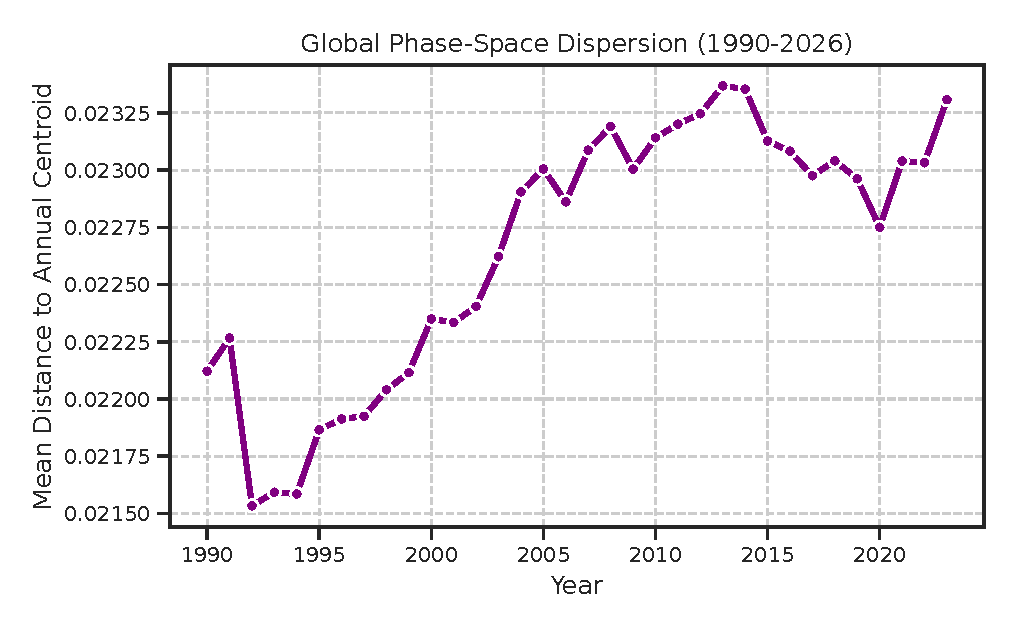
\includegraphics[width=0.75\textwidth]{../figures/fig3_global_dispersion.eps}
    \caption{\textbf{Phase-Space Dispersion Over Time.} The mean Euclidean distance of all states from the global centroid (1990--2026).}
    \label{fig:dispersion}
\end{figure}

\subsection{Data-Driven Trajectory Typologies}
Projecting 5,628 historical observations (1990--2026) onto the manifold reveals that linear development is a statistical rarity. Applying unsupervised $K$-Means clustering ($K=3$) to the log-transformed Tortuosity and Geodesic Inefficiency metrics organically identifies three distinct movement paradigms, visualized in Figure \ref{fig:trajectories}.

The first archetype, \textbf{Direct} ($N=88$), consists of states with low tortuosity and near-perfect geodesic efficiency that move purposefully toward a stable attractor, exemplified by the Dominican Republic. The second, \textbf{Meandering} ($N=67$), describes states like Mauritania that experience gradual, curving transitions; these states adhere to natural geodesic paths but take significantly longer Euclidean routes. Finally, the \textbf{Erratic} typology ($N=15$), represented by Kyrgyzstan, identifies states trapped in highly tortuous limit cycles. These cases exhibit immense Geodesic Inefficiency, indicating volatile institutional changes that repeatedly fight against the natural topology of the system.

\begin{figure}[htbp]
    \centering
    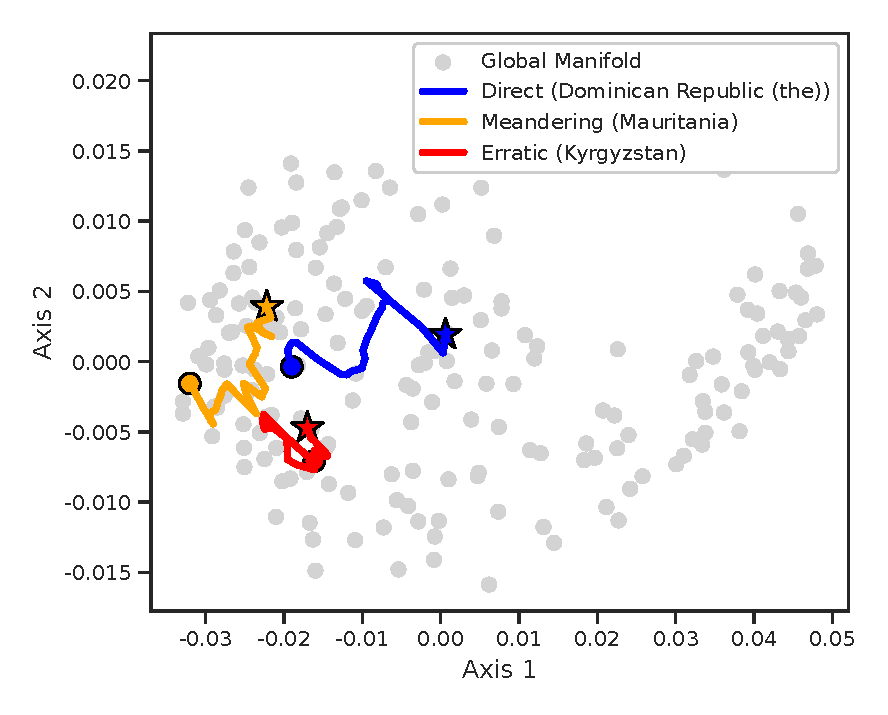
\includegraphics[width=0.65\textwidth]{../figures/fig4_trajectory_typologies.eps}
    \caption{\textbf{Governance Trajectory Typologies (1990--2026).} Historical paths illustrating Direct development (Dominican Republic, blue), Meandering transitions (Mauritania, orange), and Erratic regime cycling (Kyrgyzstan, red).}
    \label{fig:trajectories}
\end{figure}

\section{Discussion and Conclusion}

\subsection{Synthesis of Findings}
This paper introduces a novel geometric framework for analyzing the macro-historical trajectories of state development. By applying manifold learning and persistent homology to longitudinal global governance data (1990--2026), we demonstrate that state-building is neither a linear progression nor a random walk. Instead, it is constrained by a highly structured topology.

Our findings mathematically formalize the concept of developmental ``forbidden zones.'' The persistent $H_1$ loops identified via Topological Data Analysis (TDA) prove that certain configurations of governance—specifically the intersection of high structural wealth with extreme political corruption and low polyarchy—are systemically unstable. Furthermore, by calculating the Geodesic Inefficiency and Trajectory Tortuosity of 170 states, we identified three distinct paradigms of institutional evolution: Direct, Meandering, and Erratic. The disparity between these typologies reveals that a state's current static categorization (e.g., ``electoral autocracy'') is far less analytically valuable than the momentum and efficiency of its historical trajectory.

\subsection{Policy Implications: The Limits of Static Conditionality}
These geometric realities have profound implications for international development policy. Currently, institutions such as the International Monetary Fund (IMF), the World Bank, and the United Nations rely heavily on static, year-over-year indicator benchmarks to determine aid conditionality and reform targets.

This static approach often ignores the geodesic ``terrain'' of the international system. As demonstrated by the Erratic trajectory typology (exemplified by Kyrgyzstan), attempting to forcibly inject advanced democratic or economic architectures into a state without the underlying institutional geometry to support it does not accelerate development; it triggers catastrophic structural recoils. When international institutions demand reforms that push a state directly across a topological void—rather than guiding it along the natural, if meandering, geodesic pathways of the manifold—they inadvertently engineer systemic collapse. Development policy must pivot from maximizing short-term indicator growth to optimizing trajectory efficiency, minimizing the ``tortuosity'' of state-building by respecting the systemic constraints of the governance manifold.

\subsection{Methodological Limitations}
While this framework offers a robust new methodology for comparative politics, several limitations must be acknowledged. First, despite utilizing $K$-Nearest Neighbors imputation to retain autocratic regimes, the structural missingness of data in failing or highly repressive states introduces inherent approximation into the extreme edges of the manifold. Second, the underlying geometry is sensitive to hyperparameter selection, particularly the kernel bandwidth ($\epsilon$) in the diffusion map and the neighborhood size ($k$) in the geodesic graph. While our Procrustes sensitivity analysis confirms the macro-stability of our 6-variable model, micro-level trajectory variations may occur under different algorithmic specifications. Finally, the temporal scope of this study (1990--2026) captures the specific dynamics of the post-Cold War era; the topological shape of global governance during the height of the 20th century or the colonial era would likely exhibit different mathematical bounds.

\subsection{Conclusion}
The convergence hypothesis that dominated the late 20th century—the expectation that the global system would universally settle into consolidated, prosperous democracies—is not supported by the mathematical topology of the last three decades. Instead, our phase-space dispersion analysis reveals an international system that is actively polarizing into competing developmental basins.

To understand the future of global governance, political science must move beyond the taxonomy of static regime types. States are complex adaptive systems navigating a perilous mathematical landscape. By mapping the boundaries, voids, and corridors of this space, we can begin to measure not just where a nation currently stands, but the systemic forces dictating where it is inevitably being pulled.

\section*{Data and Code Availability}
The Python source code, generated figures, and full replication instructions for this analysis are publicly available on GitHub at \url{https://github.com/adibatic/governance-topology}.

\bibliographystyle{apalike}
\bibliography{references}

\end{document}